\documentclass{article}

\usepackage[french]{babel}
\usepackage[T1]{fontenc}
\usepackage{moreverb}       % verbatim with tab

\usepackage{wrapfig}
\usepackage{graphicx}
\usepackage{geometry}
\geometry{hmargin=2.5cm}
\usepackage{amsmath}
\usepackage{siunitx}

\usepackage{graphicx}
\usepackage{subcaption}
\usepackage{float}
\usepackage{hyperref}
\usepackage{setspace}
\usepackage{xcolor}
\usepackage{pdfpages}
\usepackage{enumitem}
\usepackage{lscape}

\usepackage{fancyhdr}       % en-têtes
\usepackage{lastpage}       % numéro de dernière page

\title{Systèmes logiques programmés\bigbreak \bigbreak
    \large Dossier récapitulatif\bigbreak
    \normalsize Programmation d'un générateur de signaux en assembleur sur PIC16F887\bigbreak}
\date{2020 -- 2021}
\author{Laura Binacchi}

\pagestyle{fancy}
\renewcommand\headrulewidth{1pt}
\fancyhead[L]{Laura Binacchi}
\fancyhead[C]{Systèmes logiques programmés}
\fancyhead[R]{\today}


\begin{document}
    \pagenumbering{gobble}
    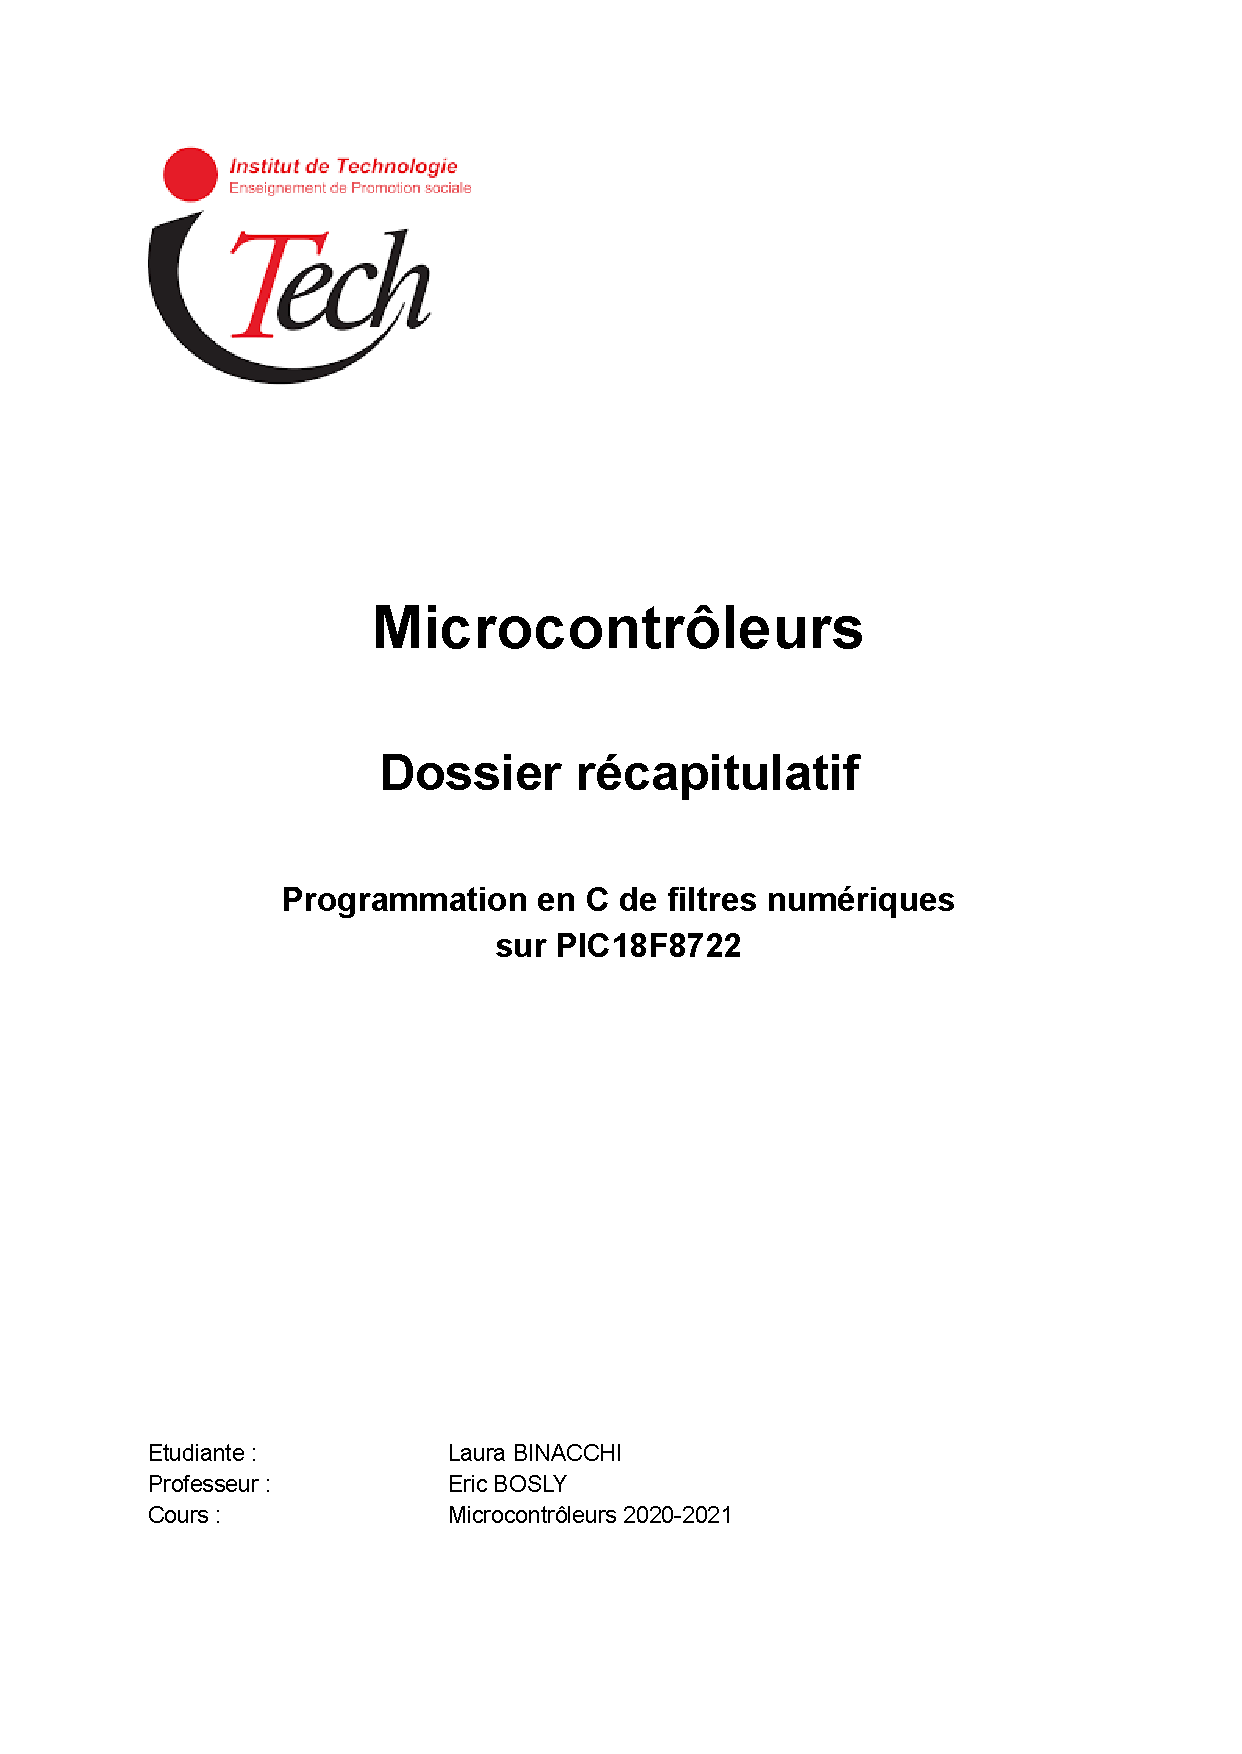
\includepdf[pages={1}]{pdg}
    \newpage
    \tableofcontents
    \newpage
    \pagenumbering{arabic}

    \section{Cahier des charges}

    \subsection{Travail demandé}
    \paragraph{}
    Ecrire un programme en langage C sous MPLABX XC8 pour filtrer un signal sonore mono envoyé à partir d’un fichier .wav sur l’entrée analogique d’un PIC. Ce programme devra tourner sur un PIC18F8722 en simulation Proteus. Ce PIC pilotera un convertisseur NA de sortie permettant d’écouter le résultat des filtres. On respectera les règles de bonne syntaxe vues au cours, notamment en termes de commentaires.

    \paragraph{}
    Un fichier Proteus d’exemple et des fichiers son ont été fournis. L’interface utilisateur du programme est laissée à l’appréciation du développeur, je propose ci-dessous un menu circulaire utilisant le LCD et des boutons poussoirs. Ne perdez cependant pas trop de temps dans ce domaine, ce n’est pas le principal. Le plus important dans ce dossier, sera la mise au point des quatre filtres demandés, programmation et tests.

    \subsection{Cahier des charges de l’application}
    \paragraph{}
    Un signal sonore en mono, généré par une application de type Audacity avec une fréquence d’échantillonnage de 8 ou 16 kHz, est injecté sur une entrée analogique du PIC. Le signal est numérisé sur 8 bits par le module CAN du PIC et filtré en temps réel selon le mode de fonctionnement courant. Le signal filtré est recomposé par un CNA MCP4922 ou DAC0808 au choix, à piloter. Le résultat est audible dans un graphe audio, exportable.

    \paragraph{}
    Connecter un afficheur LCD 4 lignes de 20 caractères, le programme aura plusieurs modes de fonctionnement, résumés dans le tableau ci-dessous.
    
    \paragraph{}
    La fréquence d’échantillonnage $F_e$ du signal sera configurable à 8kHz ou 16kHz. La fréquence d’échantillonnage conditionne évidement les fréquences de coupure des filtres.

    \paragraph{}
    Le mode « Configuration » et les menus sont laissés à l’appréciation du concepteur. Attention aux conflits potentiels entre le LCD et le convertisseur CNA, si ils utilisent tous les deux une connexion SPI.

    \subsection{Description des 4 filtres demandés}

    \begin{tabular}{l l l} 
        Variables           & Y : tampon sortie & X : tampon entrée \\
                            & N : dimension du tampon & \\
                            & A, B : coefficients & \\
                            & & \\
        Moyenne glissante   & $Y_j = \sum\limits_{i=0}^{N-1} \frac{X_{j-i}}{N}$ & pour N = 2 à 8 \\
                            & & \\
        Filtre récursif     & $Y_j = \sum\limits_{i=0}^{N-1} A_i X_{j-i} - \sum\limits_{i=1}^{N-1} B_i X_{j-i}$ & voir fichier tableur joint \\
                            & & \\
        Echo                &  $Y_j = A X_j + B X_{j-del}$ & avec $A + B = 1$ \\
    \end{tabular}

    \paragraph{}
    Le menu décrit ci-dessous est exemplatif, pour éviter de perdre trop de temps avec Proteus, vous pouvez limiter la complexité de l’interface de l’interface homme-machine.

    
    \begin{figure}[H]
        \centering
        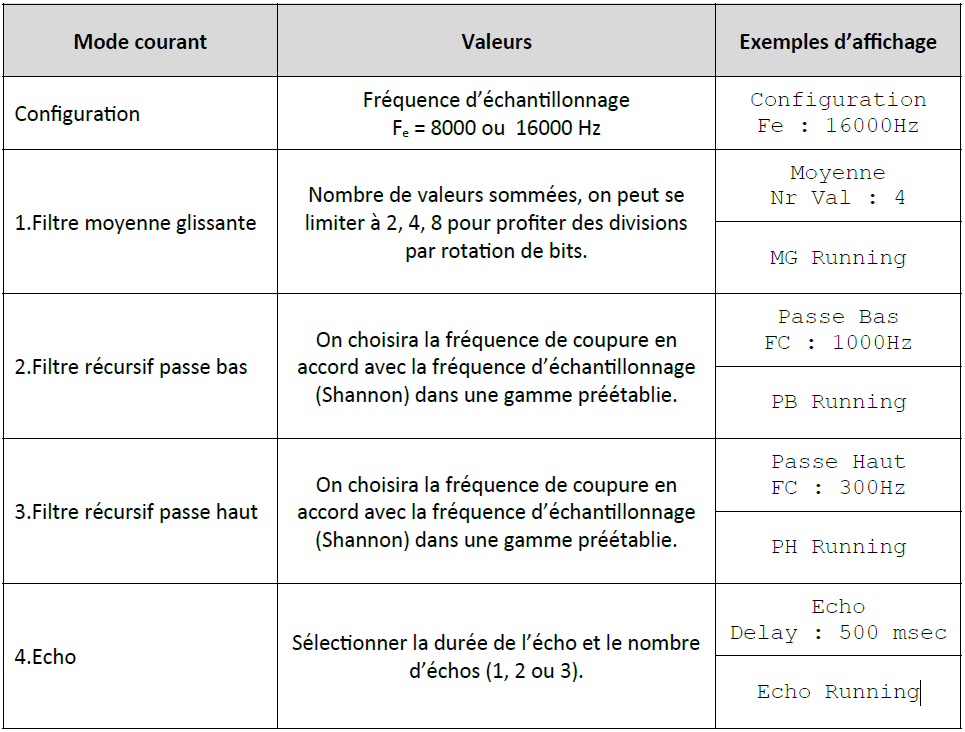
\includegraphics[width=.7\textwidth]{./images/menus.png}
    \end{figure}


    \section{Organigramme/Analyse}
    % L’organigramme de haut niveau du programme

    \section{Fréquences utilisées}
    % La description et la justification des fréquences utilisées

    \section{Configuration du PIC}
    % La description de la configuration du PIC utilisée
    DAC0808 banché directement sur le port D plutôt que via un bus de communication (SPI ou I2C) -> plus rapide -> fréquence d'échantillonnage + élevée (50 kHz au lieu de 20kHz via SPI)

    \section{Tests}
    % La description des tests à effectuer pour valider le programme

    \section{Difficultés rencontrées}

    









    \section{Analyse}
    \paragraph{}
    

    

    \section{Configuration}
    \paragraph{Conversion analogique-digitale (A/D conversion)}
    ADCON0 permet de :
    - activer la conversion (bit ADON)
    - vérifier quand la conversion est faite (bit GO/DONE)
    - sélectionner l'entrée analogique liée à l'ADC

    ADCON1 :
    permet de
    - configurer les entrées en analogique ou digital (TOR)
    Par défaut, tout est analogique. Ici on sera en 1101 (AN0 AN1), éventuellement 1011 (de AN0-3, AN2-3 étant des PIN de tension de ref) -> attention aux PIN en TOR dont on a besoin
    - configurer les tensions de référence du module ADC et d'où elles viennent
    Pour le programme, on travaille en mode 0 (mode par défaut), i.e. tensions de référence sur VDD et VSS (entre 0 et 5V)

    ADCON2
    gère le fonctionnement technique du module ADC, dont 
    - sa justification à droite ou à gauche (bit ADFM)
    - la configuration du temps d'acquisition (ACQT<2:0>)
    - la configuration de la fréquence de conversion, dérivée par rapport à la fréquence de l'oscillateur (ADCS<2:0>)

    ADRESH et ADRESL
    contiennent le résultat de la conversion


    1 Entrées analogiques ou digitales ? -< configuration de ADCON1

    2 Tensions de référence ? -> 00

    3 Temps de conversion ? il faut 12 temps TAD avant de finir la conversion et d'avoir le déclenchement du GO/DONE
    valeur min de TAD = 0,7us
    valeur de TAD fixé par le quartz et les bits ADCS<2:0> de l'ADCON2

    à 10MHz HSPLL, 1 tosc = 0,1us 
    puisqu'il faut min 0,7us => il faut choisir le 8tosc (001)

    => le temps de conversion va durer 12*8TOSC = 0,96us
    => on peut tenir une fréquence théorique max de 100kHz
    (limite théorique mais en pratique on doit aller moins vite pour garder de la puissance processeur pour autre chose)

    4 Temps d'acquisition ? ACQT<2:0>
    typiquement, dans un système qui ne fait pas que de la conversion, on le laisse à 0 parce que le temps de conversion est là en ayant fait autre chose avant.

    5 Justification de résultat ? ADFM 
    8 bits -> à gauche et on utilise que adresh
    10 bits -> à droite et on utilise adresh et l

    6 Choix du canal de conversion ? ADCON0
    Ici avec Proteus on n'est pas limité par un hardware déjà soudé

    7 Alimentation du CAN ?
    Dernière étape : activer l'ADC avec le bit ADON

    Utilisation : on met 1 dans le GO/DONE et on attend que ça saute pour avoir le résultat

    Code d'exemple
    fréquence d'échantillonnage de 20kHz






    \section{Fonctionnement du programme}



    \section{Tests}



    \section{Problèmes rencontrés}



\end{document}